\begin{figure*}[t]
\centering
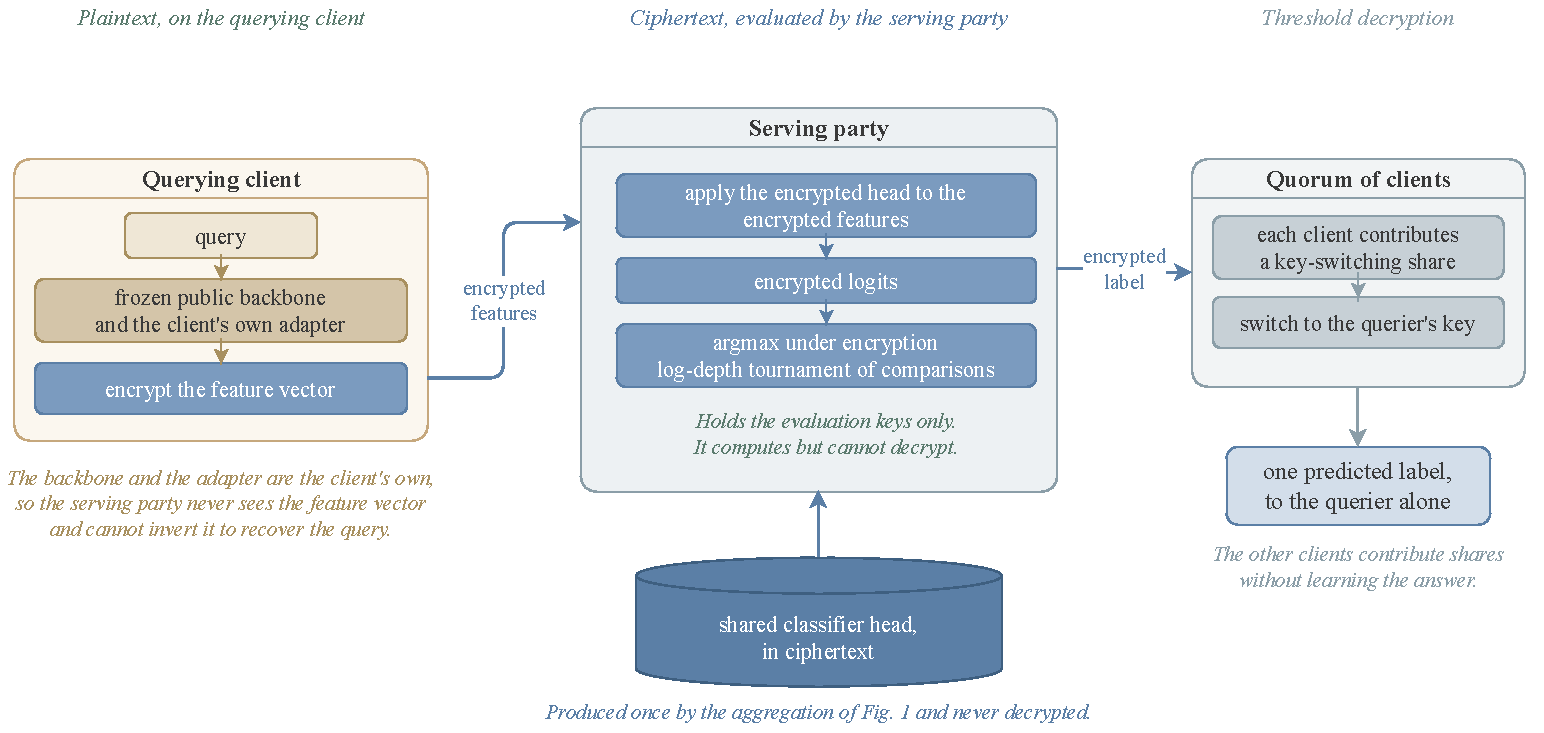
\includegraphics[width=\textwidth]{figures/fig_serving.pdf}
\caption{Answering one query. The querying client computes the features with its own backbone and adapter and encrypts them, so the server never sees the feature vector and cannot invert it to recover the query. The server holds the evaluation keys only. It applies the encrypted head, obtains encrypted logits, and reduces them to the index of the largest entry by a tournament of homomorphic comparisons. A quorum of clients then switches that index to the querying client's key, so the other clients contribute shares without learning the answer.}
\label{fig:serving}
\end{figure*}
